\chapter{Diseño}  \label{disenyo}
\section{Diseño conceptual} \label{disenyo.conceptual}


Con el análisis finalizado, el diseño de la solución prácticamente surgió por sí mismo; teniéndo en cuenta los requisitos, se llegó a la conclusión de que los desarrollos realizados a lo largo de la duración de este proyecto no serían más que el comienzo para algo mucho más grande; se debía ofrecer tanto la infraestructura necesaria como el soporte para que la solución pudiera escalar y ser expandida mediante el trabajo de futuros desarrolladores. 
\par 
El diseño conceptual del sistema se presenta a continuación a una escala abstracta y de alto nivel. Básicamente, el proyecto hará uso de numerosas fuentes de información, en este caso sobre productos fitosanitarios y sus derivados. Dicha información deberá ser recogida de manera periódica y almacenada en algún sistema de persistencia tal como proviene de sus fuentes, es decir, en una versión \textit{en crudo}. Una vez almacenada en su versión original, los datos pasarán a una siguiente fase en la que serán procesados bien para extraer la información relevante o de interés para el proyecto bien para añadir datos útiles como información de trazabilidad, todo esto con el objetivo en mente de conseguir ese esquema unificado. Una vez procesados, los datos se almacenarán en otro sistema de persistencia, o incluso en el mismo de antes, si es posible. En este punto habría dos opciones; o que los datos ya estuvieran integrados en un único modelo, o que estuvieran individualmente separados en el almacén anterior. En este segundo caso, los datos deberían ser unificados para conseguir ese esquema único y posteriormente poder ser visualizados, ya sea mediante un navegador con una aplicación web, o mediante otro método de visualización. En el diagrama de la figura \ref{fig:disenyoconceptual} se puede observar el diseño conceptual descrito anteriormente de manera gráfica. 


\begin{figure}[H]
    \centering
    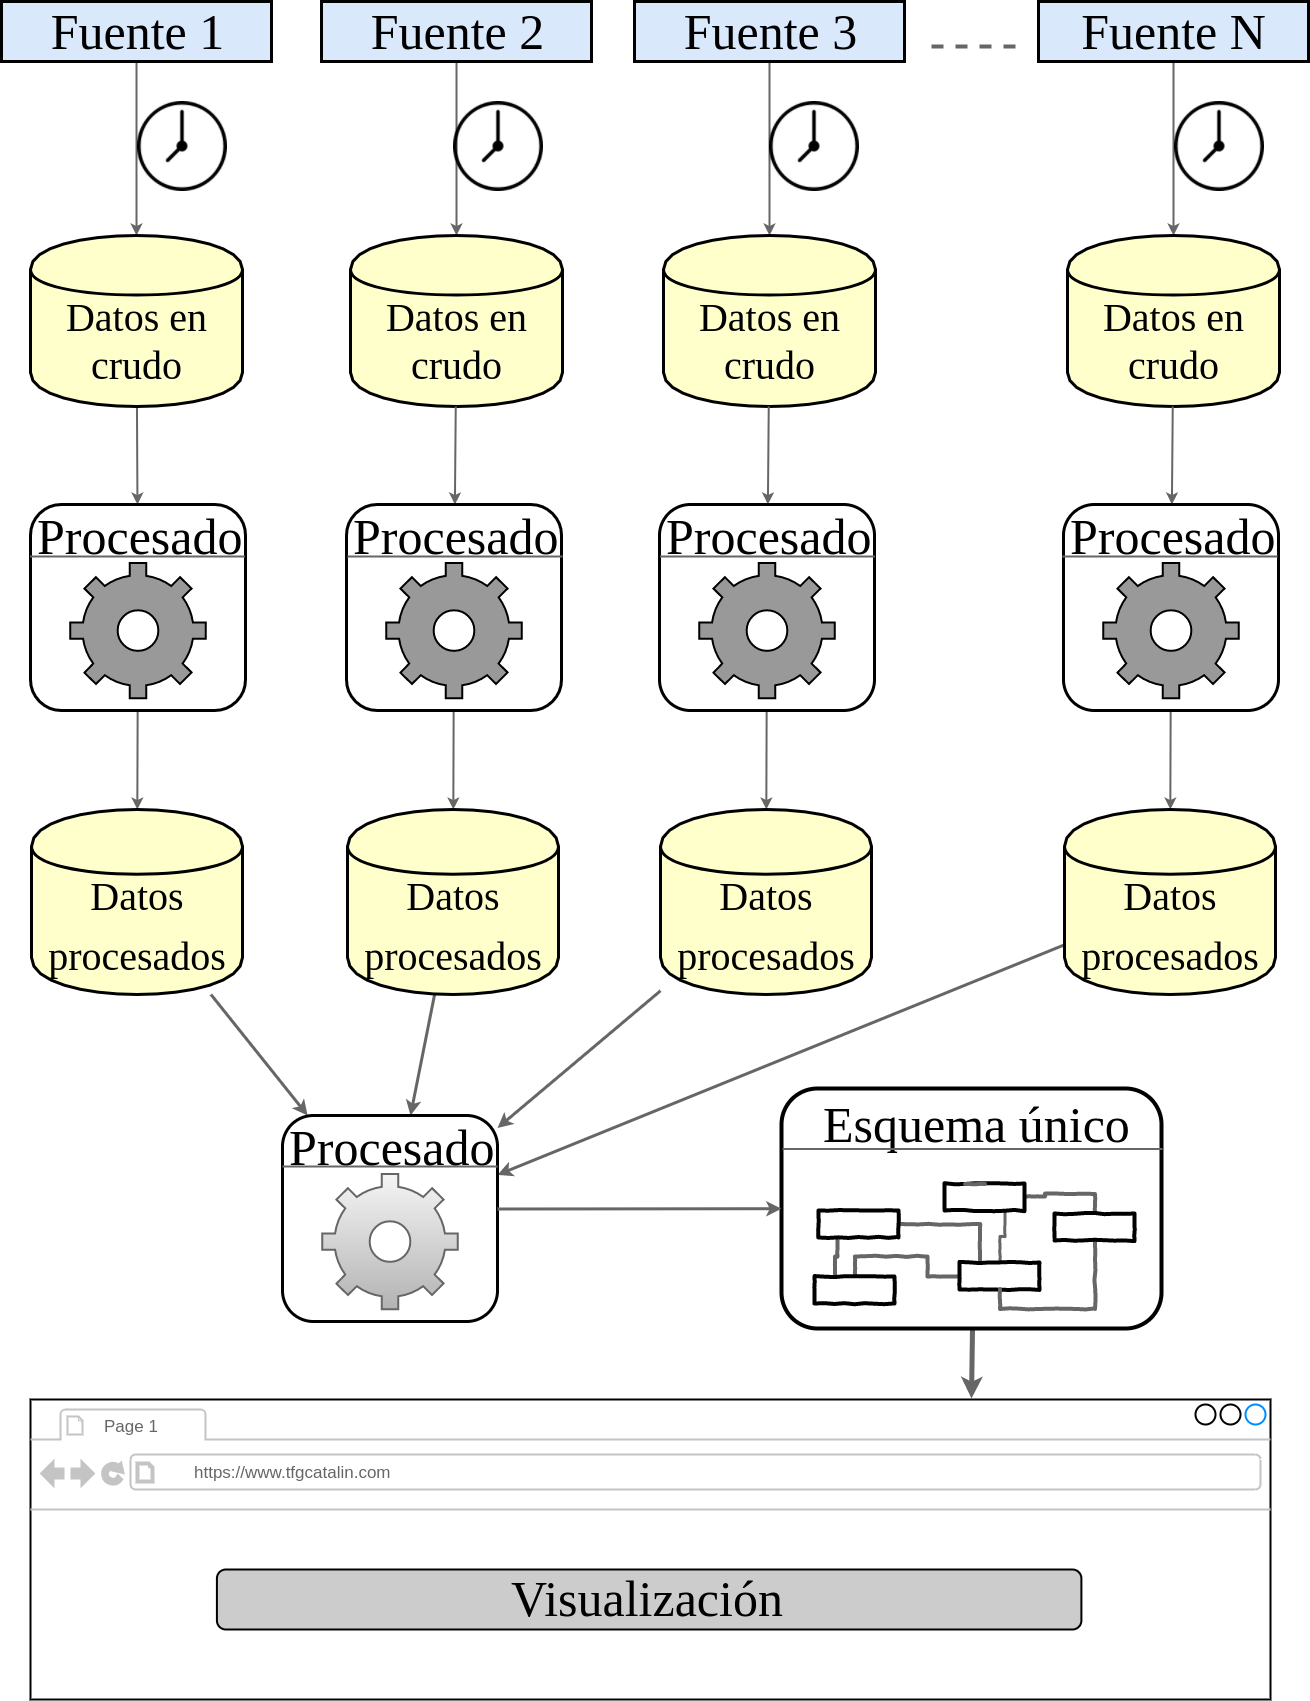
\includegraphics[width=1\textwidth,height=15cm,keepaspectratio]{Imagenes/disenyoconceptual}
    \caption{Diseño conceptual de la solución}
    \label{fig:disenyoconceptual}
\end{figure}

\section{Diseño final} \label{disenyo.final}
En el apartado anterior se ofreció una visión de alto nivel del diseño de la solución, sin hablar de herramientas ni de tecnologías concretas. En este apartado se va a profundizar en el diseño y se va a explicar en detalle la manera en que los datos pasan a través de las diferentes herramientas dentro del sistema, desde la descarga de los datos desde sus fuentes hasta su visualización en pantalla, pasándo por las diferentes etapas de procesado y almacenamiento. 
\par
En el diagrama de la figura \ref{fig:disenyofinal} se puede observar un mapeo casi dirécto entre los elementos del diseño final y los del diseño conceptual de la figura \ref{fig:disenyoconceptual}. Se puede observar que el diseño final incluye a \textit{Talend} como responsable tanto de los procesos que descargan y almacenan los \textit{datos en crudo} como de los que posteriormente procesan y almacenan los datos como \textit{datos procesados}. En cuanto al sistema de almacenamiento, que guardará tanto los datos originales como los modificados se utilizará \textit{Hadoop} para los \textit{datos en crudo} y \textit{Hive} dentro de \textit{Hadoop} para los \textit{datos procesados}. Una vez los datos estén transformados y almacenados corréctamente, se usará \textit{Sqoop} para transferirlos a ese esquema único que se persigue como objetivo, y que estará almacenado dentro de una base de datos \textit{MySQL}. Para que este último paso sea posible, debe ser el propio \textit{Talend} quien prepare los datos para ser integrados diréctamente en el esquema unificado. \textit{JHipster} tendrá una conexión directa a la base de datos \textit{MySQL} y gracias a ello será capaz de leer los datos y mostrarlos en pantalla con su propia interfaz web. 
\begin{figure}[H]
    \centering
    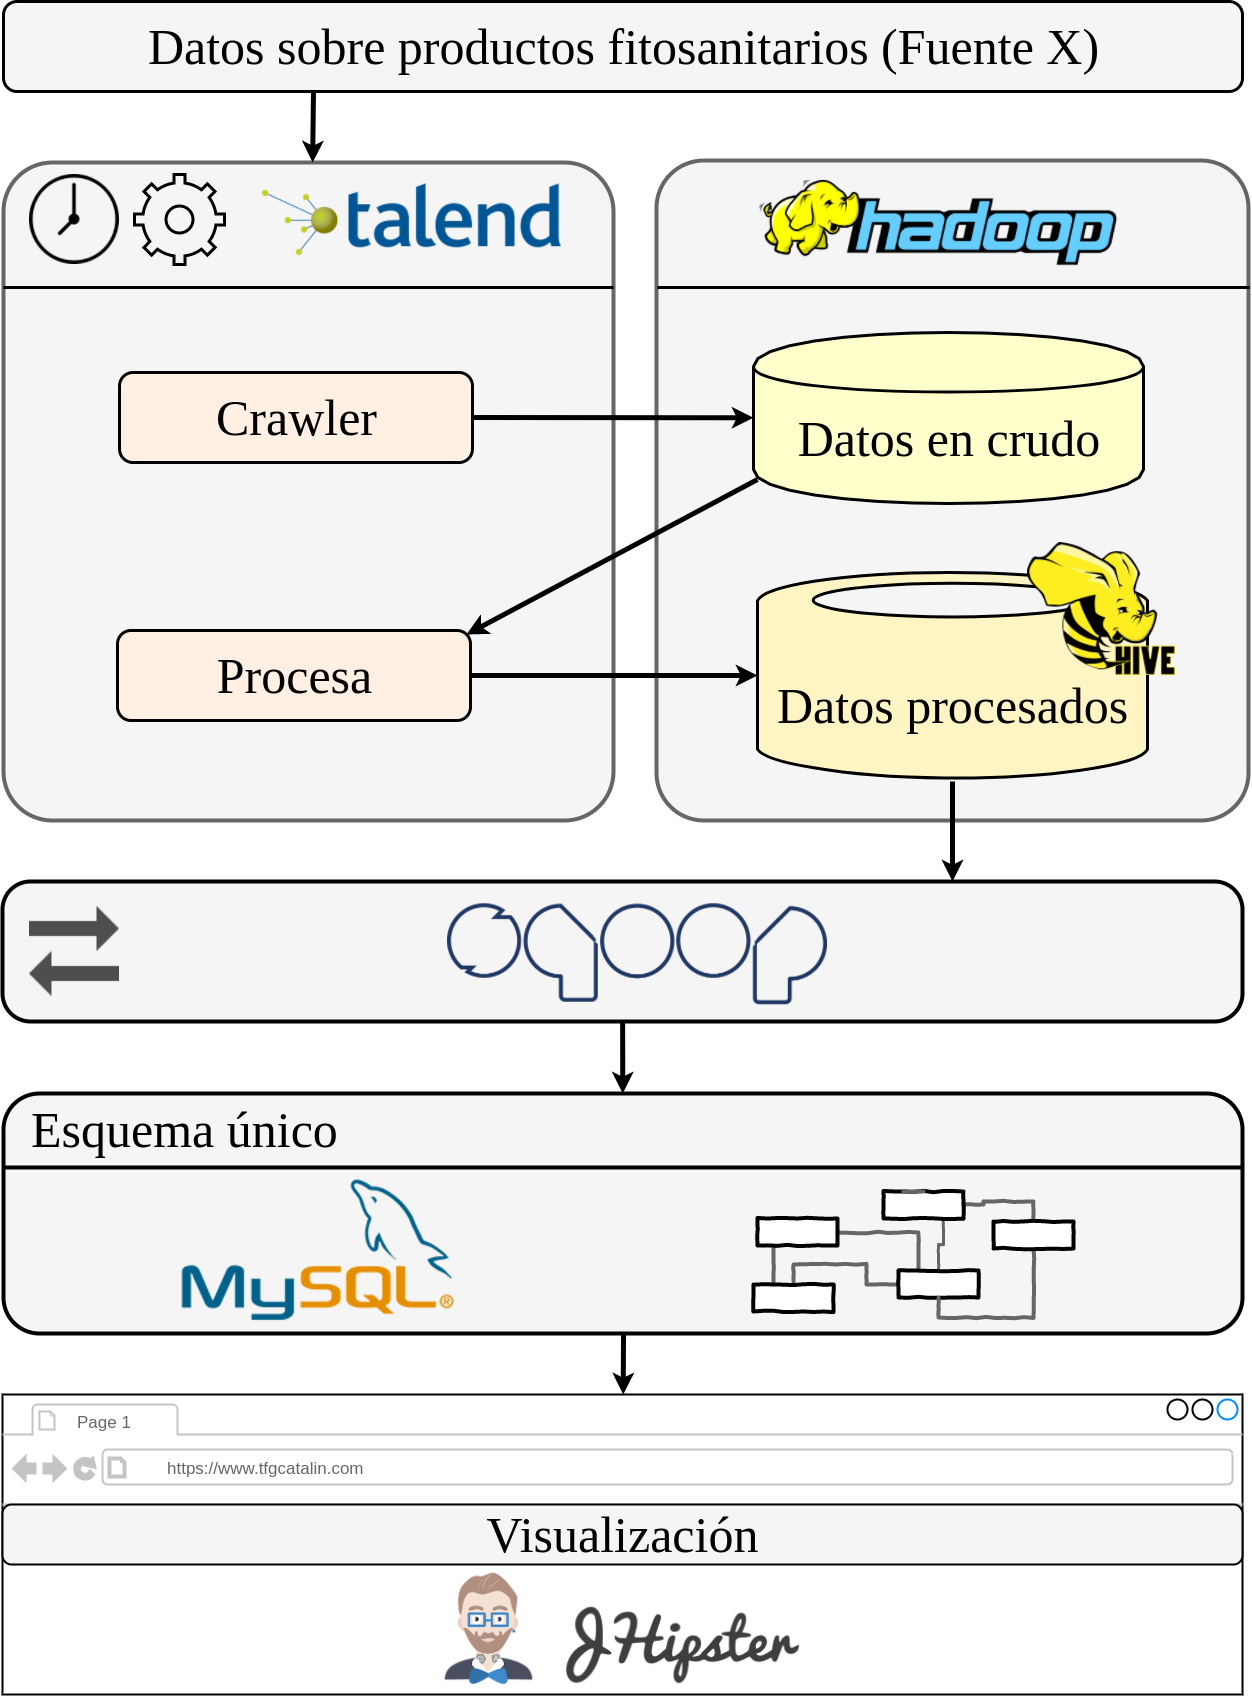
\includegraphics[width=1\textwidth,height=15cm,keepaspectratio]{Imagenes/disenyofinal}
    \caption{Diseño final de la solución}
    \label{fig:disenyofinal}
\end{figure}


\section{Arquitectura del sistema} \label{disenyo.arquitectura}
Diagramas arquitecturales, explicar los diferentes componentes y la manera en la que interaccionan y se comunican desde el momento de la recolección de los datos hasta su presentación en la aplicación final. Incluir aparte del diagrama de herramientas algun diagrama de componente y conector, e incluso algún trocito con un diagrama de flujo y a ser posible un diagrama de clases de JHipster y la manera en la que interaccionan con el sistema.
\begin{itemize}
\item \textbf{Diagrama de despliegue.}

\begin{figure}[H]
    \centering
    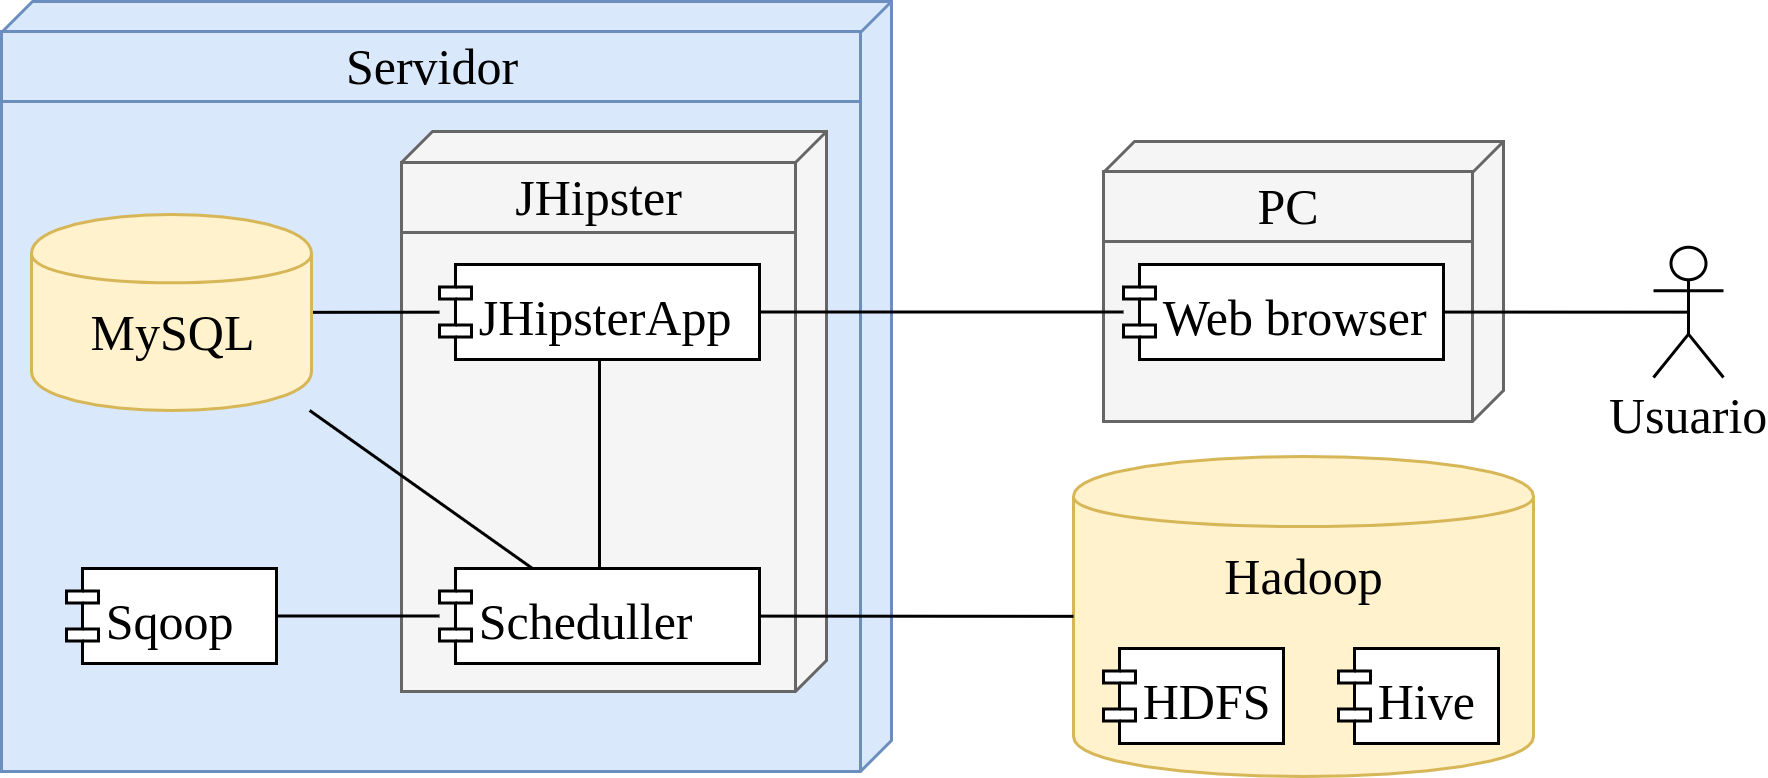
\includegraphics[width=1\textwidth,height=15cm,keepaspectratio]{Imagenes/despliegue}
    \caption{Diagrama de despliegue de la solución}
    \label{fig:despliegue}
\end{figure}


\item \textbf{Diagrama de componente y conector.}
\item \textbf{Diagrama de clases.}
\item \textbf{Diagrama de datos.}
\item \textbf{Diagrama de secuencia.}
\end{itemize}


\section{Estrategia de integración} \label{disenyo.estrategia}
